\section{Background}\label{sec:background}
% General introduction
Data demand is predicted to growth by a factor of 10 in 2020 from today's values by major network providers \cite{cisco2016forecast,kremling2015presentation,belllabs2016report,ericsson2015report}. The use of cellular networks for data consumption has become
widespread due in part to the massive increase in mobile applications and services for content delivery, e.g. Netflix, YouTube; social networking,  e.g. Facebook, Twitter, Snapchat, Instagram; and cloud computing and storage, e.g. Dropbox, OneDrive, Amazon S3, Amazon EC2. Further, content delivery networks are expected to carry three-fourths of all the Internet video traffic by the end of 2020 \cite{cisco2016forecast}. Streaming applications that are based in multicast where a transmitter needs to serve tens, hundreds or even thousands of receivers are drawing large attention in mobile networks such as \ac{LTE-A} or \ac{WLAN} networks such as \ac{WiFi}. Use cases of video streaming in highly-crowded scenarios, e.g. sports stadiums, airports, service-waiting areas or museums, are attractive but also challenging to the content providers. Serving a large amount of users with unicast schemes drain the network resources since each user needs a dedicated channel. Instead, it would be preferable a scheme where users are served in a broadcast fashion by synchronizing to it. These types of scenarios pose tight requirements to ensure a satisfactoring \ac{QoE} for all the users. First, video services require high throughput and low delay to avoid stalling events in the end-user device. Second, to cope with the users data load, a high-capacity access network is required to accomodate all the users. Third, an efficient transmission schemes are required to serve them as quick as possible. To address these requirements, service providers should utilize 4G high-capacity mobile networks or \ac{WiFi} networks using a broadcast scheme to serve all the users.

For the network operator, techniques that can offload the service infrastructure in a multicast network to cope with such data load, are needed in order to satisfy the overall demand and reduce the energy consumption at the \ac{BS}. Further, given that all end-users experience different channel conditions in such scenario, there might exist users with a degraded connection to a \ac{BS} that increase the delay and reduce the throughput. Instead, a better connectivity might be provided by other users either within the cellular spectrum or through a \ac{WiFi} network. However, the management of mobile devices without good cellular coverage but with access to this local network can potentially be decentralized.

For the mobile user, device internal energy consumption has become a limiting factor in terms of battery life due to data transmissions. Without a transmission scheme properly designed for reduced delay and high throughput, energy consumed by data transmissions can drain the mobile device battery reducing the time that a device request a service. Besides data transmissions, mobile devices perform much more internal tasks than older devices from ten years ago and since energy has become critical for the users \cite{fitzek2007mobile,ravi2008context,perruci2009energy}.

Therefore, mobile network designers need to consider mechanisms and techniques that aim for high throughput and low energy consumption both at the station and the end user devices and that are able to provide data offloading from current network infrastructures. An effective solution to this problem is to consider cooperation between the devices. This approach exploits short-range communication protocols between the mobile devices, e.g. \ac{WiFi}, Bluetooth and more recently \ac{D2D} in \ac{LTE-A} within the cellular spectrum, to offload the network and improve the mentioned metrics.

\subsection{Cooperative Wireless Networks}
% Cooperation
The concept of cooperation in wireless networks has been investigated before \cite{fitzek2006cooperation,fitzek2007cognitive,fitzek2013mobile}. The main goal is to diminish the amount of communications resources (data rate, energy or even storage and computational power) to convey an information of common interest from a transmitter to a set of interconnected receivers in a multicast fashion. Devices connected in this way form a \textit{mobile cloud} \cite{fitzek2013mobile}. In these prior works, cooperation through \ac{WiFi} or Bluetooth for the short-range was always preferable than broadcast in former 2.5G and 3G cellular networks since the data rates for the short-range were much higher than the cellular ones. However, the appearance of \ac{D2D} in \ac{LTE-A} calls this assumption into question since both cellular and short range data rates are comparable. Therefore, it is required to understand when does cooperation becomes a better choice than broadcast for these scenarios in terms of rate and energy costs. In Fig.~\ref{fig:cooperation}, it can be observed a comparison example of no cooperation and cooperation in a multicast wireless network.

\begin{figure}[ht!]
  \centering
  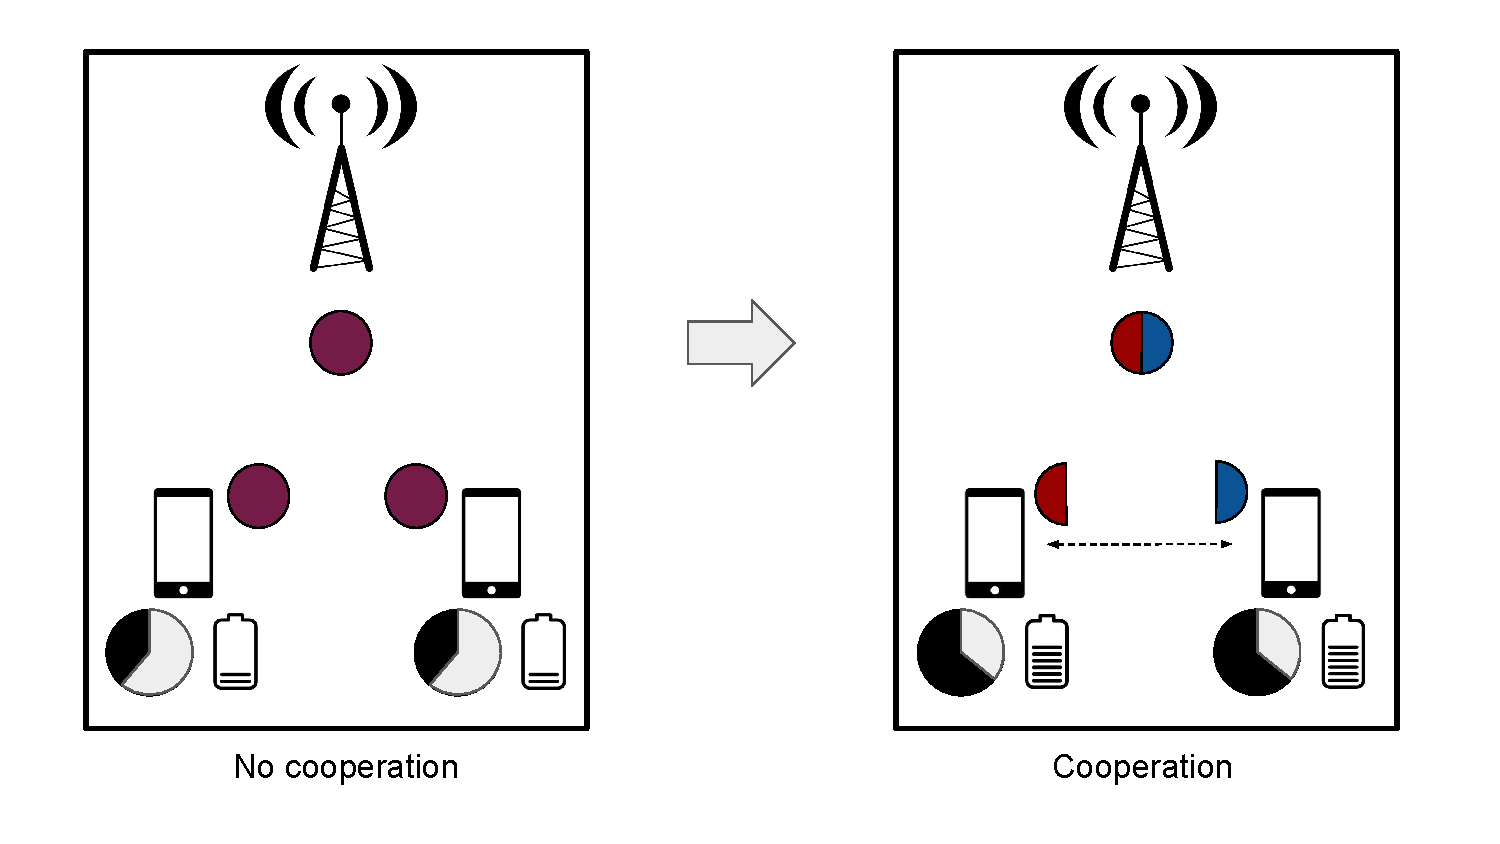
\includegraphics[width=\textwidth]{introduction/figures/cooperation.pdf}
  \caption{Cooperation in Wireless Networks.}
\label{fig:cooperation}
\end{figure}

Without cooperation, a purple content is sent to two mobile devices in a broadcast fashion. This requires a large downloading time and energy expenditure to send two copies of the content (one to each device) and ensure both devices are satisfied. When cooperation is considered, the content now is split into smaller blue and red pieces where each of them is sent rapidly to each device. Thus, half the cellular resources are used in this example. Then, the devices exploit short-range communications (dashed line) by exchanging their missing pieces. The key underlying idea is for the devices share their missing information through a faster, short-distance and reliable link where data rate and energy costs are expected to be higher than in the cellular network. This increases the total throughput and reduces the overal energy consumption since the time and energy to distribute the information is reduced. From an operator perspective, the information \textit{as a whole} is quickly disseminated into the receivers helping the \ac{BS} to offload data. At the end, the goal of reducing the use communication resources at the \ac{BS} is achieved. In this way, mobile clouds allow to improve the overall network performance and user experience.

\subsection{Device to Device Communications in Mobile Networks}
\label{sec:d2d}
One of the key aspects to achieve the gains proposed by the cooperative approach is the short-range technology to be considered and its parameters to guarantee a fast and reliable link. Besides \ac{WLAN} technologies like \ac{WiFi}, there has been a large interest in \ac{D2D} communications integrated into \ac{LTE-A} \cite{lin2013comprehensive,asadi2014survey,feng2014device,tehrani2014device}. This permits the devices to share data without going through the \ac{BS} network which keeps the idea of data offloading. The work in \cite{asadi2014survey} proposes a classification of \ac{D2D} communications. First, according to its spectrum use, the communications could be in the cellular network (inband) or outside in a local network (outband). Second, for inband \ac{D2D} the communications could take place in the spectrum of other mobile users (underlay) or another dedicated only to \ac{D2D} (overlay). Second, for outband \ac{D2D}, the coordination between cellular and local network radio interfaces is either controlled by the cellular \ac{BS} (controlled) or the users themselves (autonomous). For network assisted or inband \ac{D2D}, authors in \cite{fodor2014design} review the key challenges to enable \ac{D2D} services. Device discovery, communications resource allocation and coordination for these type of communications are handled by the cellular network. Furthermore, \ac{D2D} based \ac{ProSe} have been included in \cite{3gpp2012prose} to use them in \ac{LTE-A} networks for an improved \ac{QoE}.

\subsection{Erasure Correcting Codes for Multicast Networks}
\label{sec:erasure_codes}
Another aspect that is relevant for cooperation gains in multicast scenarios is channel coding. The dynamics of the wireless medium, propagation conditions, noise and interference may degradate the received \ac{SINR} thus making reception unfeasible for some period of time. In the case of packet networks, this leads to \textit{erasure} channels where packets are either correctly received or lost. Therefore, to protect against packet erasures, some redundancy is added with an erasure correcting code. They are relevant to make multicast applications reliable since error protection mechanisms with feedback based on retransmissions, e.g. \ac{ARQ}, are very costly in the case of multiple users. For example, if we consider a multicast scenario with a 1\% packet loss rate for all the links when transmitting 100 packets to 1000 users, this means that with high probability all data packets would need to be sent again at least once more time plus the required \ac{ACK} packets. However, adding 10\% or less redundancy might be sufficient to complete the transmission of missing packets to all receivers. Thus, \ac{ARQ} based schemes with feedback control through \ac{ACK} packets are not possible for a large number of devices.

Different erasure correcting codes might be used for reliable multicast applications. In the literature, we can find linear block codes such as \ac{RS} \cite{reed1960polynomial} or \ac{LDPC} \cite{gallager1962low}. These codes fix the amount of redundancy to be generated for error correction from the original data through a \textit{code rate} which depends on the packet loss rate. Still, if the packet loss rate varies they may generate too much redundancy or even not be able to correct erasures. More recently, \ac{LT} codes \cite{luby2002lt} and Raptor codes \cite{shokrollahi2006raptor} are more adaptable to the channel conditions than block codes since they always generate redundancy regardless of the channel conditions, thus being called \textit{rateless} codes. These latter type of codes are characterized by being: (i) able to generate a large number of coded symbols due to the rateless property, (ii) close-to-optimal, requiring a slightly higher amount of encoded symbols than the original set to decode, and (iii) able to decode with a subset of coded symbols as long as there are no inter-dependencies in it. These erasure correction properties among others have led to consider Raptor codes its standardization in multicast \ac{LTE-A} networks through the \ac{eMBMS} protocol \cite{embms2011general}. Later, RaptorQ codes from Qualcomm \cite{qualcomm2011raptorq} were proposed as an extension of Raptor codes.

Although these coding techniques are useful for multicast networks, they pose two major restrictions to apply them in a cooperative approach. First, this type of coding is made on a \textit{end-to-end} basis, meaning that for each hop encoding and decoding is required to be made before sending coded packets to the next hop. The required code processing for each hop increases the delay and energy consumption due to computational costs \cite{toemoeskoezi2015packet}. Second, as a consequence of the previous, these codes are not composable. Although there has been constructions composable rateless codes, e.g. distributed \ac{LT} codes \cite{puducheri2006distributed}, its operational conditions are very restrictive and thus, impractical in general. This implies there are no practical forms to create new coded packets from packets that have been coded previously without decoding in the case of rateless codes. Because of these limitations state of the art rateless codes are not ideal erasure correcting codes for cooperative wireless networks with \ac{D2D} due to the inherent processing in multihop.

\subsection{Network Coding for Multicast Networks}
% Network Coding, inter-session (XOR) and intra-session (RLNC)
Introduced by Alshwede et al. \cite{ahlswede2000network}, \ac{NC} appeared as an effective technology to remove the limitations presented previously. In this work, the authors presented a new paradigm shift for conveying information in communication networks. Instead of treating the packets as atomic, unmodifiable units at the intermediates node in a network, they are regarded as algebraic elements in a \ac{GF} that can be operated on to create new coded packets. \ac{RLNC} \cite{ho2006random} was introduced by Ho et al. In this scheme, coded packets are algebraic linear combinations of original set of packets from a single data flow. This type of coding can be made across any node in the network. Further, \ac{RLNC} is proven to achieve the multicast capacity from a flow perspective with very high probability \cite{koetter2003algebraic,ho2006random}. In this way, instead of typically encoding and decoding on a hop-by-hop basis, as it would happen with other erasure codes, coding is performed on a \textit{network} basis. Relaying nodes can recode packets to reduce delay and still take advantage of the data representation for the next hop. Also, recoding can occur with partial information, meaning that as packets are received from a previous hop without decoding. In this sense, \ac{RLNC} appears as the only coding technique that overcomes the restrictions mentioned earlier in Section~\ref{sec:erasure_codes}.

\begin{figure}[h]
  \centering
  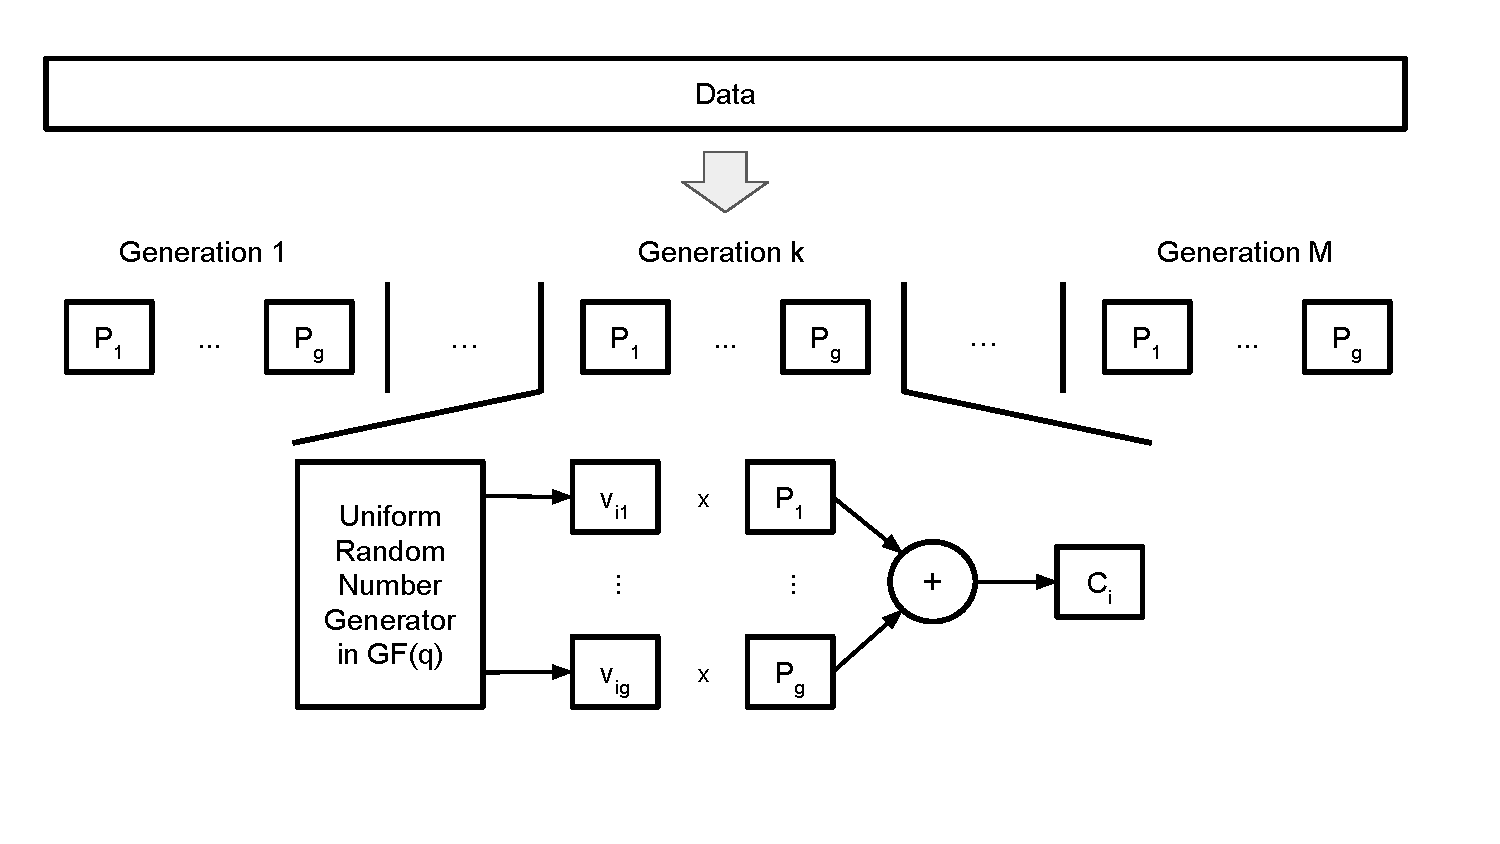
\includegraphics[width=\textwidth]{introduction/figures/RLNC.pdf}
  \caption{RLNC encoding process.}
\label{fig:rlnc_enc}
\end{figure}

As seen in Fig.~\ref{fig:rlnc_enc}, in \ac{RLNC} the information to be transmitted is split into packets which are grouped into sets called \textit{generations} \cite{chou2003practical}. Each generation $k = 1, \ldots, M$ consists of $g$ original packets $P_i,\ i = 1, \ldots, g$ used to create new coded packets as with any \ac{FEC} technique from Section~\ref{sec:erasure_codes}. For each generation, each coded packet generated is a linear combination of all the original packets $C_i = \sum_{j = 1}^g v_{ij} P_j,\ i \geq 1$. Here, $v_{ij}$ is the coding coefficient that multiplies packet $j$ in the process of creating packet $i$. The coefficients are picked uniformly at random from $GF(q)$ where $q$ is the field size. All the operations are properly defined under the arithmetics of $GF(q)$.

After creating a coded packet, it is necessary to signal the coding coefficients utilized for encoding to the decoder. The signalling method that guarantees potential recoding without major caveats, is to append each coding coefficient used to create that coded packet as overhead. For each coded packet there is an overhead of $|v_{i}| = \sum_{j = 1}^g \log_{2}(q) = g \times \log_{2}(q),\ [bits]\ \forall i$. To get the original packets, a decoder only needs to collect \textit{any} set of $g$ linearly independent coded packets to create a $g \times g$ matrix with the coding coefficients and perform Gaussian elimination \cite{fragouli2006network} to solve the linear equations made in the encoding process.

Despite being a relatively recent technology, practical applications of \ac{RLNC} started to appear a few years after its inception. The work of Chachulski et al. in 2007 considered \ac{MORE} \cite{chachulski2007more}, the first protocol using \ac{RLNC} which showed different achievable gains in real wireless mesh networks. Different areas with \ac{RLNC} use cases can also be found in \cite{fragouli2006network}. Also, \ac{RLNC} has found applications in areas such as: \ac{P2P} networks \cite{gkantsidis2005network}, distributed storage \cite{dimakis2010network} and network coding based \ac{TCP} \cite{kim2014modeling}. Moreover, standard software libraries have appeared such as Kodo \cite{kodo2011pedersen}, a network coding C++11 library whose purpose is to ease the development of protocols using \ac{RLNC}.

\subsection{Related Work}

For reliable multicast, various works have been made to quantify the gains of broadcast with \ac{RLNC} against other transmission schemes in terms of erasure codes, feedback possibility and transmission policies. Among these, it can be mentioned: throughput and delay gains of reliable multicast with \ac{RLNC} \cite{eryilmaz2008delay}, time division duplexed channels \cite{lucani2009random,lucani2009queue}, (implementation on real devices \cite{heide2009network} and protocols with resource allocation of multicast \ac{RLNC} based networks \cite{vukobratovic2014random,chiti2013optimized,tassi2015resource}. Similar to fountain rateless codes, the key underlying idea is that \ac{RLNC} creates indistingueshable coded packets helping many receivers to recover different lost packets at the same time. At the end, this capability helps all the end-users to obtain the required data much faster increasing the throughput.

Different from other erasure correcting codes, \ac{RLNC} is well-suited for multicast cooperative networks due to its recoding capability. Using \ac{RLNC} allows to create recoded packets \textit{on-the-fly}, meaning as soon as previously encoded packets are received at a node. \ac{RLNC} does not incur in processing delays required by decoding and encoding new packets such as conventional erasure correcting codes mentioned earlier. This feature has made \ac{RLNC} an alternative in other works that employ the cooperative approach. Studies that have considered multicast cooperative mobile clouds with \ac{RLNC} have been related to: cooperative mobile clouds for energy reduction \cite{heide2012green}, social mobile \ac{D2D} clouds \cite{fitzek2013implementation} and optimal transmission policies for broadcast and cooperation between unicast \ac{D2D} pairs \cite{khamfroush2013minimizing,khamfroush2015optimal}. Although very diverse, these studies have focused mostly in \ac{D2D} pairs or standard \ac{RLNC} solutions while omitting posible improvements both allowing the devices to multicast and considering alternate code constructions. Moreover, these studies assume that the \ac{D2D} links are faster which could not be the case with new advances in mobile networks.

\clearpage
